%! Author = Omar Iskandarani
%! Date = 2/15/2025

\documentclass[aps,preprint,superscriptaddress]{revtex4}

\usepackage{array}
\usepackage{booktabs}
\usepackage{amsmath}
\usepackage{amssymb}
\usepackage{graphicx}
\usepackage{hyperref}
\usepackage{physics}

\begin{document}
\sloppy % Allow LaTeX to adjust spacing to avoid overfull boxes
\author{Omar Iskandarani}
\title{The Vortex Æther Model: Æther Vortex Field Model}
\date{\today}
\affiliation{Independent Researcher, Groningen, The Netherlands}
\thanks{ORCID: \href{https://orcid.org/0009-0006-1686-3961}{0009-0006-1686-3961}}
\email{info@omariskandarani.com}


%%%%%%%%%%%%%%%%%%%%%%%%%%    Abstract    %%%%%%%%%%%%%%%%%%%%%%%%%%


\begin{abstract}
    The Vortex Æther Model (VAM) introduces a unified, non-relativistic framework wherein gravity, electromagnetism, and quantum phenomena emerge from structured vorticity in an inviscid superfluid-like æther. Unlike General Relativity, which invokes spacetime curvature, VAM models stable vortex knots in a 3D Euclidean medium with absolute time. Observed time dilation results from vortex-induced local energy gradients. This paper derives time dilation analogs to GR, explores vortex-energetic time shifts, and presents experimental implications.
\end{abstract}


\maketitle
%%%%%%%%%%%%%%%%%%%%%%%%%%    Introduction    %%%%%%%%%%%%%%%%%%%%%%%%%%
\newpage

    \begin{figure}[h]
        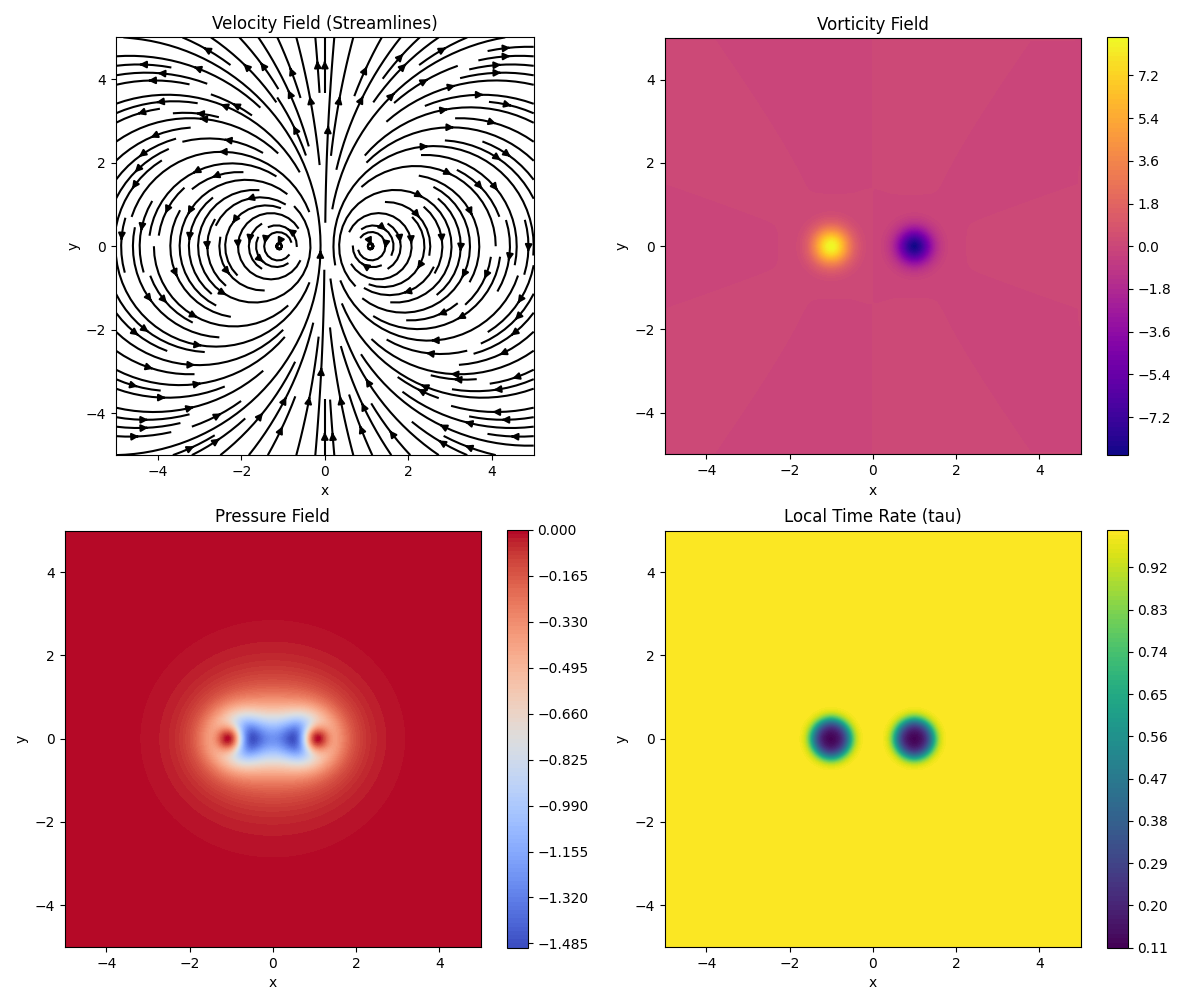
\includegraphics[width=\textwidth]{vorticity_field1}
        \caption{Illustration of vorticity fields in Æther.}
        \label{fig:vorticity_field1}
    \end{figure}

    \section*{Core Assumptions}
    The Æther is modeled as an inviscid, incompressible superfluid governed by:

\begin{tabular}{ll}
    \toprule
    \midrule
        * & Conservation of Absolute Vorticity \\
        * & A 3D Euclidean medium with absolute time \\
        * & Particles as vortex knots \\
        * & Irrotational outside vortex cores, but with conserved vorticity inside knots \\
        * & Gravity from vorticity-induced pressure gradients \\
    \bottomrule
\end{tabular}

    Let:

    \begin{tabular}{ll}
        \toprule
        Symbol & Description \\
        \midrule
        \(\vec{v}\) & Æther velocity field \\
        \(\vec{\omega}\) &  Vorticity \(\vec{\omega} = \nabla \times \vec{v}\) \\
        \(\rho_\text{æ}\) & Æther density (constant) \\
        \(\Phi\) & Vorticity-induced potential \\
        \(\kappa\) & Circulation constant \\
        \(\mathcal{K}\) & Knot topological class (Hopf link, torus knot, etc.) \\
        \bottomrule
    \end{tabular}

    \subsection*{Introduction to Fluid Dynamics and Vorticity Conservation}
    Euler Equation (Inviscid Flow)
    \begin{equation}
        \frac{\partial \vec{v}}{\partial t} + (\vec{v} \cdot \nabla)\vec{v} = -\frac{1}{\rho_\text{æ}} \nabla p
    \end{equation}
    Taking the curl to get the Vorticity Transport
    \begin{equation}
        \frac{\partial \vec{\omega}}{\partial t} + (\vec{v} \cdot \nabla)\vec{\omega} = (\vec{\omega} \cdot \nabla) \vec{v}
    \end{equation}

    \subsection*{Vorticity-Induced Gravity}
    We define a Newtonian like vorticity-based gravitational potential $\Phi$:
    \begin{equation}
        \vec{F}_g = -\nabla \Phi
    \end{equation}
    Where $\Phi$ is the Vorticity Potential:
    \begin{equation}
        \Phi(\vec{r}) = \gamma \int \frac{|\vec{\omega}(\vec{r'})|^2}{|\vec{r} - \vec{r'}|} \, d^3r'
    \end{equation}
    This mirrors the Newtonian potential but replaces mass density with vorticity intensity. This gives attractive force fields between vortex knots (like a particle).



%%%%%%%%%%%%%%%%%%%%%%%%%%    PART 1    %%%%%%%%%%%%%%%%%%%%%%%%%%
%! Author = mr
%! Date = 3/27/2025

\section{Time Dilation in the Æther-Vortex Model}\label{sec:Part-1}
We consider an inviscid, irrotational superfluid æther with stable topological vortex knots. The Æther experiences absolute time $t_{\text{abs}}$, but local clocks experience slowed rates due to pressure gradients and knot energetics. The Vortex Æther Model posits that the rate at which time flows in the local frame (near the knot) depends on the internal angular frequency $\Omega_k$. In this section, we derive time dilation analogues inspired by the predictions of general relativity (GR), based solely on pressure and vorticity gradients in the fluid.

\subsection{Bernoulli-Based Local Time Modulation}
In high-vorticity regions, Bernoulli's principle implies a drop in pressure near vortex cores:
\begin{equation}
    \frac{1}{2} \rho_\text{æ} v^2 + p = p_0 \Rightarrow p = p_0 - \frac{1}{2} \rho_\text{æ} v^2
\end{equation}
Assuming that the local physical clock rate is proportional to pressure, we define the local frequency of time as:
\begin{equation}
    f_{\text{local}} = f_0 \cdot \left( \frac{p}{p_0} \right) = f_0 \left( 1 - \frac{\rho_\text{æ} v^2}{2p_0} \right)
\end{equation}
Thus, the dilation of local time relative to absolute (background) time becomes:
\begin{equation}
    \frac{t_{\text{local}}}{t_0} = \left( 1 - \frac{\rho_\text{æ} v^2}{2p_0} \right)^{-1}
\end{equation}
For circular vortex flow where $v = \Omega r$:
\begin{equation}
    \frac{t_{\text{local}}}{t_0} \approx 1 + \frac{\rho_\text{æ} \Omega^2 r^2}{2p_0}
\end{equation}
This reduces time rate locally with higher knot rotation, modeling time modulation without relativity, where $\rho_\text{æ}/p_0 \sim 1/c^2$.

\subsection{Heuristic Time Modulation by Knot Rotation}
Let $\Omega_k$ be the average angular velocity of a vortex knot:
\begin{equation}
    \label{eq:omegamod}
    \frac{t_{\text{local}}}{t_{\text{abs}}} = \left(1 + \alpha \Omega_k^2 \right)^{-1}
\end{equation}
For small $\Omega_k$:
\begin{equation}
    \frac{t_{\text{local}}}{t_{\text{abs}}} \approx 1 - \alpha \Omega_k^2 + \mathcal{O}(\Omega_k^4)
\end{equation}
This matches special relativistic time dilation:
\begin{equation}
    \frac{t_{\text{moving}}}{t_{\text{rest}}} \approx 1 - \frac{v^2}{2c^2}
\end{equation}
This heuristic expression generalizes the local effect of rotational energy into a topological time-modulation law, consistent with the Bernoulli-derived expansion in the low-vorticity limit.

\subsection{Vorticity-Induced Gravitational Time Dilation}
In the æther-vortex framework, gravity emerges from pressure gradients induced by localized vorticity.
Let $\Phi(\vec{r})$ be a scalar potential analogous to the Newtonian gravitational potential, defined by:
\begin{equation}
    \Phi(\vec{r}) = \gamma \int \frac{|\vec{\omega}(\vec{r}')|^2}{|\vec{r} - \vec{r}'|} \, d^3r'
\end{equation}
Time dilation follows:
\begin{equation}
    \frac{t_{\text{local}}}{t_{\infty}} = \sqrt{1 - \frac{2\Phi(\vec{r})}{c^2}}
\end{equation}
High vorticity → low pressure → slowed time
If the vorticity field is concentrated at a point-like knot (analogous to a mass), i.e., $|\vec{\omega}(\vec{r}')|^2 \sim \delta(\vec{r}')$, we retrieve a Newtonian-like form:
\begin{equation}
    \frac{t_{\text{local}}}{t_{\infty}} = \sqrt{1 - \frac{2\gamma \omega_0^2}{r c^2}}
\end{equation}

\subsection{Kerr-Like Time Adjustment}
From GR:
\begin{equation}
    t_{\text{adjusted}} = \Delta t \cdot \sqrt{1 - \frac{2GM}{rc^2} - \frac{J^2}{r^3 c^2}}
\end{equation}
In Æther terms:
\begin{equation}
    \boxed{t_{\text{adjusted}} = \Delta t \cdot \sqrt{1 - \frac{\gamma \langle \omega^2 \rangle}{r c^2} - \frac{\kappa^2}{r^3 c^2}}}
\end{equation}
This reproduces gravitational and frame-dragging effects via vorticity and circulation.

\subsection{Conclusion and Experimental Outlook}
The Vortex Æther Model replaces spacetime curvature with conserved vorticity in a 3D fluid. Time dilation arises from localized pressure depletion and kinetic energy storage within vortex knots, offering a classical, topological reinterpretation of relativistic effects. In this formulation, time slows in regions of high vorticity due to pressure depletion, aligning with relativistic predictions \cite{fedi2017gravity, simula2020gravitational, winterberg1990maxwell}. Future work includes simulations of vortex clocks and tests using BECs, helium II, or electrohydrodynamic lifters.



%%%%%%%%%%%%%%%%%%%%%%%%%%    PART 2    %%%%%%%%%%%%%%%%%%%%%%%%%%
\subsection*{Section II: Time Modulation by Vortex Knot Rotation}

Building upon the previous section's treatment of time dilation via pressure and Bernoulli dynamics, we now focus on the intrinsic rotation of topological vortex knots. In the Vortex Æther Model (VAM), particles are modeled as stable, topologically conserved vortex knots embedded in an incompressible, inviscid superfluid medium. Each knot possesses a characteristic internal angular frequency $\Omega_k$, and this internal motion induces local time modulation relative to the absolute time of the æther.

Rather than curving spacetime, we propose that internal rotational energy and helicity conservation induce temporal slowdowns analogous to gravitational redshift. This section develops these ideas through heuristic and energetic arguments consistent with the hierarchy introduced in Section I.

\subsection*{A. Heuristic and Energetic Derivation}

We begin by proposing a rotationally-induced time dilation formula based on the knot's internal angular frequency:

\begin{equation}
\frac{t_{\text{local}}}{t_{\text{abs}}} = \left(1 + \alpha \Omega_k^2 \right)^{-1}
\end{equation}

where:

\begin{itemize}
\item $t_{\text{local}}$ is the proper time near the knot,
\item $t_{\text{abs}}$ is the absolute time of the background æther,
\item $\Omega_k$ is the average core angular frequency,
\item $\alpha$ is a coupling coefficient with dimensions $[\alpha] = \text{s}^2$.
\end{itemize}

For small angular velocities, we obtain a first-order expansion:

\begin{equation}
\frac{t_{\text{local}}}{t_{\text{abs}}} \approx 1 - \alpha \Omega_k^2 + \mathcal{O}(\Omega_k^4)
\end{equation}

This form parallels the Lorentz factor at low velocities in special relativity:

\begin{equation}
\frac{t_{\text{moving}}}{t_{\text{rest}}} \approx 1 - \frac{v^2}{2c^2}
\end{equation}

This establishes an important analogy: internal rotational motion in VAM induces temporal slowing, similar to how translational velocity induces time dilation in SR.

To strengthen the physical foundation of this expression, we now relate time dilation to the energy stored in vortex rotation. Let the vortex knot have an effective moment of inertia $I$. Its rotational energy is given by:

\begin{equation}
E_{\text{rot}} = \frac{1}{2} I \Omega_k^2
\end{equation}

Assuming time slows due to this energy density, we write:

\begin{equation}
\frac{t_{\text{local}}}{t_{\text{abs}}} = \left(1 + \alpha E_{\text{rot}} \right)^{-1} = \left(1 + \frac{1}{2} \alpha I \Omega_k^2 \right)^{-1}
\end{equation}

This expression serves as the energetic analog of the pressure-based Bernoulli model from Section I. It supports the interpretation of vortex-induced time wells via energy storage rather than geometric deformation.

We highlight this key result with a boxed formulation:

\begin{equation}
\boxed{\frac{t_{\text{local}}}{t_{\text{abs}}} = \left(1 + \frac{1}{2} \alpha I \Omega_k^2 \right)^{-1}}
\end{equation}

\subsection*{B. Topological and Physical Justification}

Topological vortex knots are not only characterized by rotation but also by helicity:

\begin{equation}
H = \int \vec{v} \cdot \vec{\omega} \, d^3x
\end{equation}

Helicity is a conserved quantity in ideal (inviscid, incompressible) fluids, encoding the linkage and twisting of vortex lines. The rotational frequency $\Omega_k$ becomes a topologically meaningful indicator of the knot’s identity and dynamical state.

Higher $\Omega_k$ implies greater rotational energy and stronger localized pressure depletion, forming a "temporal well" in the æther. These wells naturally mimic gravitational redshift effects in curved spacetime, but arise here purely from classical fluid mechanics.

This model:

\begin{itemize}
\item Attributes time modulation to conserved, intrinsic rotational energy,
\item Requires no external reference frames (absolute æther time is universal),
\item Preserves temporal isotropy outside the vortex core,
\item Provides a natural replacement for GR's spacetime curvature.
\end{itemize}

Therefore, this vortex-energetic time dilation principle provides a powerful alternative to relativistic time modulation by anchoring all temporal effects in rotational energetics and topological invariants.

In the next section, we will show how these ideas reproduce metric-like behavior for rotating observers, including a direct fluid-mechanical analog to the Kerr metric of General Relativity.
%%%%%%%%%%%%%%%%%%%%%%%%%%    PART 3    %%%%%%%%%%%%%%%%%%%%%%%%%%
%! Author = mr
%! Date = 3/27/2025

\section{proper time for a rotating observer}\label{sec:Part-3}

In General Relativity, the flow of proper time for a rotating observer in a stationary, axisymmetric spacetime is given by
\begin{equation}
    \left(\frac{d\tau}{dt}\right)^2_{\text{GR}} = -\left[g_{tt} + 2 g_{t\phi}\Omega_{\text{eff}} + g_{\phi\phi}\Omega_{\text{eff}}^2\right],
    \label{eq:GRtime}
\end{equation}
where $\Omega_{\text{eff}}$ is the observer's angular velocity, and the metric components $g_{\mu\nu}$ describe spacetime curvature (e.g., Kerr geometry) \cite{misner1973gravitation}.

In a vortex-based Æther theory, we posit that time dilation arises not from spacetime curvature, but from the local motion of an inviscid superfluid medium. We associate metric-like effects with Æther flow variables:
\begin{align*}
    g_{tt} &\rightarrow -\left(1 - \frac{v_r^2}{c^2} \right), \\
    g_{t\phi} &\rightarrow -\frac{v_r v_\phi}{c^2}, \\
    g_{\phi\phi} &\rightarrow -\frac{v_\phi^2}{c^2} r^2,
\end{align*}
where $v_r$ and $v_\phi$ are the radial and tangential components of Æther velocity, and $v_\phi = r \Omega_k$, with $\Omega_k = \kappa / (2\pi r^2)$ representing the local vortex rotation rate \cite{fedi2017gravity, sbitnev2021quaternion}.

Substituting into the structure of Equation~\ref{eq:GRtime}, we obtain:
\begin{align}
    \left( \frac{d\tau}{dt} \right)^2_{\text{Æther}} &= 1 - \frac{v_r^2}{c^2} - 2\frac{v_r v_\phi}{c^2} - \frac{v_\phi^2}{c^2} \\
    &= 1 - \frac{1}{c^2}(v_r + v_\phi)^2 \\
    &= 1 - \frac{1}{c^2}(v_r + r \Omega_k)^2.
    \label{eq:timeflow}
\end{align}

This result mirrors the GR proper time flow structure, yet is entirely fluid-mechanical. It predicts the slowing of proper time near intense vortex structures due to Æther flow speeds approaching $c$, effectively creating a “time-well” analogous to gravitational redshift.

\subsection*{Kerr-Like Time Adjustment from Vorticity and Circulation}

The General Relativistic form of time adjustment near a rotating mass, such as in the Kerr geometry, is approximately
\begin{equation}
    t_{\text{adjusted}} = \Delta t \cdot \sqrt{1 - \frac{2GM}{rc^2} - \frac{J^2}{r^3 c^2}}.
    \label{eq:kerrtime}
\end{equation}

We now express this in Æther-vortex terms, replacing $M$ and $J$ with effective vorticity energy density and circulation:
\begin{itemize}
    \item Mass-energy term: $\displaystyle \frac{2GM}{rc^2} \rightarrow \frac{\gamma \langle \omega^2 \rangle}{rc^2}$,
    \item Angular momentum term: $\displaystyle \frac{J^2}{r^3 c^2} \rightarrow \frac{\kappa^2}{r^3 c^2}$.
\end{itemize}

Thus, the Æther-based analog becomes:
\begin{equation}
    \boxed{
        t_{\text{adjusted}} = \Delta t \cdot \sqrt{
            1 - \frac{\gamma \langle \omega^2 \rangle}{r c^2}
            - \frac{\kappa^2}{r^3 c^2}
        }
    }
    \label{eq:ae_kerr}
\end{equation}

This formulation reproduces gravitational and frame-dragging time effects purely from Æther dynamics: $\langle \omega^2 \rangle$ plays the role of gravitational redshift, and circulation $\kappa$ encodes rotational drag. This approach aligns with recent fluid-dynamic interpretations of gravity and time \cite{barcelo2011analogue}, \cite{fedi2017gravity}.



%%%%%%%%%%%%%%%%%%%%%%%%%%    References    %%%%%%%%%%%%%%%%%%%%%%%%%%

    \bibliography{citations}
    \bibliographystyle{apsrev4-2}



%%%%%%%%%%%%%%%%%%%%%%%%%%    Appendices    %%%%%%%%%%%%%%%%%%%%%%%%%%

    \appendix \label{sec:Part-4}
    \section{Appendix}

\subsection*{I. Vortex Knots as Particles}
Each particle is a topological vortex knot:
\begin{itemize}
    \item Charge ↔ twist or chirality of knot
    \item Mass ↔ integrated vorticity energy
    \item Spin ↔ knot helicity:
\end{itemize}
\subsection*{Helicity as Particle Identity}
\begin{equation}
    \mathcal{H} = \int \vec{v} \cdot \vec{\omega} \, d^3x
\end{equation}
Stability ↔ knot type (Hopf links, Trefoil, etc.) and energy minimization in the vortex core

\subsection*{II. Vortex Thread Interaction}
Interactions arise from exchange of vorticity or reconnections between vortex filaments:
\begin{itemize}
    \item Attractive if threads reinforce circulation (parallel)
    \item Repulsive if threads cancel (antiparallel)
    \item Interaction strength:
\end{itemize}
\begin{equation}
    \vec{F}_{\text{int}} = \beta \cdot \kappa_1 \kappa_2 \cdot \frac{\vec{r}_{12} \times (\vec{v}_1 - \vec{v}_2)}{|\vec{r}_{12}|^3}
\end{equation}
Where \(\kappa_i\) are circulations of filaments and \(\vec{r}_{12}\) is the vector between them.


\subsection*{III. Thermodynamic & Quantum Behavior from Vorticity Fluctuations}
\begin{itemize}
    \item Entropy \(\leftrightarrow\) volume of vortex expansion or knot deformation
    \item Quantum transitions \(\leftrightarrow\) topological reconnection events
    \item Zero-point motion \(\leftrightarrow\) background quantum turbulence of the Æther:
\end{itemize}
\subsection*{Quantum Vorticity Background}
\begin{equation}
    \langle \omega^2 \rangle \sim \frac{\hbar}{\rho_\text{æ} \xi^4}
\end{equation}
Where \(\xi\) is the coherence length between vortex filaments
\label{appendix:1}

\end{document}